\chapter{CESM Experiments}
\label{chap:cesm-runs}
In order to examine the sensitivity of cross-equatorial flow on the strength of lateral friction, I have conducted a multitude of different numerical experiments using the \ac{CESM}. This chapter describes how their parameters have been modified (\secref{sec:cesm-setup}), and then summarizes the observations I have made during post-processing (\secref{sec:cesm-evaluation}).

It is found that while lowering viscosity may introduce a considerable amount of numerical noise (\secref{sec:cesm-noise}), the overall structure of the global circulation stays mostly intact, with the only difference that equatorial circulations now extend further to the East (\secref{sec:obs-global}). Lower equatorial viscosities indeed lead to a weaker overturning in the Atlantic\sidenote{By \(\lesssim \SI{1.5}{\sv}\) or about \SI{10}{\percent}.} (\secref{sec:obs-amoc}). For extreme viscosity modifications, the structure in the equatorial layer is changed drastically, featuring strong re-circulation cells and zonal jets. These re-circulations cause a considerable fraction of water to cross the equator in the eastern part of the basin (up to half of the total transport). The \ac{ITF} shows a similar signal (\secref{sec:obs-itf}): Overall transports vary by about \SI{10}{\percent}, while the structure of the flow is strongly altered. Extreme viscosity modifications cause flow in the \ac{NGCUC} to feed the \ac{ITF} instead of retroflecting into the \ac{NECC}, causing an increase of salinity in the throughflow region\sidenote[-4]{This is only the case in \grid{x3}, while the path of the \ac{NGCUC} is largely unaltered in \grid{x1} due to a different geometry of the \ac{ITF} region in this grid.}.

After observing that the \ac{ITF} transport and especially its composition seem to depend critically on viscosity, \secref{sec:island-rule} reviews some implications on the applicability of the \q{Island Rule}. The Island Rule was introduced in \cite{godfrey}, and predicts the flow around an island based on the wind stress to its east, which is often applied to estimate the \ac{ITF}. Since the Island Rule does not account for friction, the observed fluctuations of the \ac{ITF} cast some doubt whether it is valid close to the equator. An extension of the Island Rule including frictional effects by \citet{wajsowicz} predicts a \emph{lower} \ac{ITF} transport for \emph{higher} viscosities, in contrast to the observed behavior.

\clearpage
\section{Experimental Setup}
\label{sec:cesm-setup}
Each simulation is integrated forward for 100 years until the spin-up process is largely complete and a steady circulation has been achieved. Unless specified otherwise, all further analysis is carried out on a 20-year average of the \ac{CESM} output (years 80--99). All parameters not related to horizontal friction are left at their default value, apart from the fresh water restoring parameter \verb|sfwf_weak_restore| that is set to a value of \num{0.55}, which leads to a more realistic magnitude of the \ac{AMOC}.

The viscosity structure of the various \ac{CESM} experiments\sidenote{With friction parameterization and viscosity parameters as described in \secref{sec:cesm-friction}.} has been altered in three different ways:
%
\begin{enum}
	\item Global scaling of the parameters;
	\item Regional scaling of the parameters (\ie only in the boundary layer, or only in the interior); and
	\item Latitude-dependent%
	\sidefigure{Scaling factor of the boundary layer viscosity in the cosine-banded runs.}[fig:cosband]%
	{\importpgf{figures/cesm/}{visc-profile.pgf}}[1]%
	scaling of the boundary layer viscosity \(\nu_M\), modulated with a cosine-shape:
	\begin{equation}
	\nu_M \to \begin{cases}
	\nu_M \left(1 - \cos^2\left(\frac{\pi}{2}\frac{\theta}{\theta_L}\right)\right) & \text{if } \abs{\theta} \leq \theta_L \\ \nu_M & \text{else}
	\end{cases}
	\end{equation}
	%
	with a parameter \(\theta_L\) denoting the latitude where the Munk layer viscosity approaches its unmodified value (\figref{fig:cosband}). The boundary layer viscosity is thus reduced to the background value at the equator in these runs.
\end{enum}
%
\tabref{tab:runs} gives an overview of the \ac{CESM} simulations that I have conducted. The resulting viscosity of all runs as output by \ac{CESM} is shown in \appendixref{sec:viscosity-all}. 

Note that not all experiments are equally \q{interesting} --- some runs, like \run{x3_x1visc} or \run{x3_lowvisc_interior} are merely included as control runs, and are omitted from parts of the evaluation to follow if they did not show any interesting dynamics. Likewise, the experiments that merely form a ramp of the parameter \(\theta_L\) (\ie \run{x3_lowvisc20} -- \run{x3_lowvisc60}, and eventually \run{x3_nomunk}) often just show a gradual shift towards some behavior. In this case, not all of these experiments are mentioned explicitly during evaluation.

\begin{table}
	\begin{whole}
	\begin{tabular}{p{5ex}@{}lp{2ex}@{}ll}
		& \sfcaps{Viscosity structure} & & \sfcaps{Parameter} & \sfcaps{Identifier} \\[1.5ex]
		%
		%\cmidrule{2-5}
		%
		& default & & --- & \run{x3_default} \\
		%
		& & & \ang{\pm 20} lat.& \run{x3_lowvisc20} \\ 
		& & & \ang{\pm 30} lat.& \run{x3_lowvisc30} \\ 
		& & & \ang{\pm 45} lat.& \run{x3_lowvisc45} \\ 
		& \multirow{-4}{*}{cosine banded \(\nu_M\)} & \ldelim\{{-4}{*}& \ang{\pm 60} lat.& \run{x3_lowvisc60} \\
		%
		& no Munk layer (\(\nu_M=0\)) & & --- & \run{x3_nomunk} \\
		%
		& & & \num{0.1} & \run{x3_lowvisc_global} \\
		& \multirow{-2}{*}{linearly scaled \(\nu_A\), \(\nu_B\), \(\nu_M\)}& \ldelim\{{-2}{*} & \num{4} (\(\nu_A, \nu_B\)), \num{2} (\( \nu_M \))& \run{x3_hivisc} \\
		%
		& linearly scaled \(\nu_A\), \(\nu_B\) & & \num{0.1} & \run{x3_lowvisc_interior} \\
		%
		\ldelim\{{-10}{*}[\grid{x3}\hspace*{1ex}] & all as in \run{x1_default} & & --- & \run{x3_x1visc} \\[1.5ex]
		%
		%
		& default & & --- & \run{x1_default} \\
		& & & \num{0.5} & \run{x1_halfmunk} \\
		\ldelim\{{-3}{*}[\grid{x1}\hspace*{1ex}] & \multirow{-2}{*}{linearly scaled \(\nu_M\)} & \ldelim\{{-2}{*} & \num{0.1} & \run{x1_tenthmunk}
	\end{tabular}
	\end{whole}
	\caption[\ac{CESM} run overview.]{\ac{CESM} run overview. Runs are grouped by resolution, structure of viscosity modification, and extent of modification (\enquote{parameter}).}
	\label{tab:runs}
\end{table}

\clearpage
\section{Analysis}
\label{sec:cesm-evaluation}
\subsection{Numerical Noise}
\label{sec:cesm-noise}
%
\begin{figure}
	\centering
	\importpgf{figures/cesm/noise/}{noise.pgf}
	\caption[The generation of numerical noise at the equator in low viscosity \acs{CESM} experiments.]{By lowering equatorial viscosities, the solution becomes dominated by numerical noise. Shown here: data from \run{x3_lowvisc60}. The oscillating pattern in (a) can effectively be removed by smoothing with a triangular filter in zonal direction (b). The difference between the original and grid-level smooth fields is then identified as noise (c). Noise is preferably created in zonal direction, since \(\updel x > \updel y\) at the equator. Although noise actually dominates the solution in the equatorial band in \run{x3_lowvisc60}, the smoothed field is still a decent representation of the real dynamics (d).}
	\label{fig:noise}
\end{figure}%
%
By lowering the Munk layer viscosity parameter \(\nu_M\) in most runs%
\sidenote{This is the case for:\\
	\run{x3_lowvisc20} \\ \run{x3_lowvisc30} \\ \run{x3_lowvisc45} \\ \run{x3_lowvisc60} \\ \run{x3_nomunk} \\ \run{x3_lowvisc_global} \\ \run{x3_x1visc} \\ \run{x1_halfmunk} \\ \run{x1_tenthmunk}%
}, small-scale noise is introduced into the solution that may become dominant in some simulations (\figref{fig:noise}). Since this noise is effectively removed by applying a simple boxcar filter in zonal direction, I conclude that it is indeed acting on grid scale, and thus identify it with numerical (dispersive) noise (see also \secref{sec:noise}).

The generation of excessive numerical noise in the equatorial band is understandable when looking at the grid Reynolds numbers in this region. \citet{bryanvisc} give a condition of
%
\begin{equation}
\text{Re} \lesssim 2, \label{eq:noise-re-limit}
\end{equation}
%
\postquote{jochum}{\slshape so that noise advected into a grid cell is effectively diffused}. A general formulation of the Reynolds number reads
%
\begin{equation}
\text{Re} = \frac{U L}{A_H},
\end{equation}
%
with typical velocity and length scales \(U\) and \(L\), and viscosity \(A_H\). Since numerical noise is created at grid scale, I approximate the Reynolds number for this noise as
%
\begin{equation}
\text{Re}_n = \frac{\max\left(u \updel x, v \updel y\right)}{B}.
\end{equation}
%
Calculating \(\text{Re}_n\) shows that \eqref{eq:noise-re-limit} is generally fulfilled in the western boundary regions in \run{x3_default}, but not in, \eg, \run{x3_lowvisc60}  (\figref{fig:reynolds}). Instabilities that are created in the eastern parts of the equatorial regions, which are then advected westwards by Rossby waves, can thus not be diffused effectively, and the observed oscillatory patterns emerge as shown in \figref{fig:noise}.
%
\begin{figure}
 	\importpgf{figures/cesm/re-comp/}{re-comp.pgf}
 	\caption[Grid-scale Reynolds numbers in the low-viscosity runs.]{Lowering the Munk layer viscosity parameter leads to infeasibly high grid-scale Reynolds numbers in the equatorial boundary layers.}
 	\label{fig:reynolds}
\end{figure}

Since grid-scale noise may not only lead to an inaccurate solution, but also cause \emph{more} effective friction for \emph{lower} viscosities\sidenote[-1]{Recall that \(\vec{\mathcal{F}} \sim A_H \nabla^2 \vec{u}\), hence large oscillations as seen in \figref{fig:noise} may cause \(\nabla^2 u\) to negate the effect of a smaller viscosity \(A_H\), and lead to a locally larger friction term.}, results for particularly noisy runs should generally be interpreted with care. However, after comparing the smoothed velocity field of a low-viscosity run to \run{x3_default} (\figref{fig:noise}), it seems that the smoothed solution is still a reasonable representation of the real dynamics.

\clearpage
\subsection{Overall Circulation}
\label{sec:obs-global}
The large-scale, vertically integrated circulation as given by the \ac{BSF} seems largely unaffected by viscosity modifications. However, in the equatorial regions, it shows some interesting features (\figref{fig:bsf-comp-global-x3}). The \ac{NECC} gets considerably stronger in all oceans, and reaches much further east in the Atlantic and Indian oceans, to the point that an eastern boundary current begins to form. In the Indopacific region, the total magnitude of the \ac{SEC} and \ac{NEC} transports increase by at least \SI{6}{\sv} each. An increase in total transport is also observed in the North Atlantic circulation.

Thus, it seems that local viscosity changes in the equatorial region indeed have mostly local effects. The regions affected most are the equatorial Atlantic and Indopacific. Hence, these two regions are examined in detail during the following sections.

In contrast to the behavior observed in the \grid{x3} runs, viscosity modifications on the \grid{x1} grid barely seem to have any effect on the global circulation patterns (\figref{fig:bsf-comp-global-x1}). The largest changes are found around Indonesia, and along boundary currents (such as the Kuroshio, the Gulf Stream, and the Agulhas Current). A more localized analysis is required in order to detect subtle changes in the circulation.

\begin{figure}[bp]
	\begin{sidecaption}[Global \acp{BSF} for the \grid{x1} runs.]{Using the \grid{x1}-grid, the global circulation patterns seem mostly unaffected by viscosity modification. Top: \ac{BSF} in \run{x1_default}. Bottom: \ac{BSF} difference compared to \run{x1_default}. Note the very different color scales.}[fig:bsf-comp-global-x1]
		\antimpjustification
		\importpgf{figures/cesm/bsf-comp/}{bsf-comp-x1.pgf}
	\end{sidecaption}
\end{figure}

\begin{figure}
	\begin{whole}
	\importpgf{figures/cesm/bsf-comp/}{bsf-comp-x3.pgf}
	\end{whole}
	\caption[Global \acp{BSF} for the \grid{x3}-runs.]{By reducing the equatorial Munk layer viscosity, the equatorial circulation extends all the way to the eastern boundary. Shown are contours of the \ac{BSF} and the associated transport in \si{\sv}.}
	\label{fig:bsf-comp-global-x3}
\end{figure}

\clearpage
\subsection{AMOC}
\label{sec:obs-amoc}
Conveniently,%
\sidetable[Change of Atlantic cross\hyp{}equatorial transport (in Sverdrup) in \ac{CESM} experiments compared to their respective default.]{Change of Atlantic cross\hyp{}equatorial transport (in Sverdrup) in \ac{CESM} experiments compared to their respective default. Rough estimates from deeply penetrating streamlines in the vertical stream function (\figref{fig:bsf-comp-global-x3}). Uncertainties are of the order \(\pm\SI{0.5}{\sv}\).}[tab:amoc-change]{%
	\begin{tabular}{lS[table-format=1.1]}
		\run{x3_lowvisc20} & 0. \\
		\run{x3_lowvisc30} & 0. \\
		\run{x3_lowvisc45} & -0.5 \\
		\run{x3_lowvisc60} & -1. \\[1ex]
		\run{x3_nomunk} & -1.5 \\
		\run{x3_lowvisc_global} & -1. \\
		\run{x3_lowvisc_interior} & 0. \\
		\run{x3_x1visc} & -0.5 \\
		\run{x3_hivisc} & 0.5 \\[1ex]
		\run{x1_halfmunk} & -0.5 \\
		\run{x1_tenthmunk} & -0.5
	\end{tabular}
}[0]%
the vertical stream function of the \ac{AMOC} \(\Psi_A\) is written by \ac{CESM} in every time step as a diagnostic. This variable gives the meridional overturning transport in a depth-latitude slice (such that \((\Psi_A)_z = -V\), \((\Psi_A)_y = W\) with zonally integrated velocities \(V, W\)). For a circulation like the \ac{AMOC} where poleward and equator-ward flow are clearly separated in depth through the formation of \ac{NADW}, this is a very useful diagnostic, since it allows us to quantify the total cross-equatorial transport in the Atlantic at a glance.

The vertical stream function reveals a weakening of the cross-equatorial transport in the runs with extreme viscosity reductions by about \(\SI{1.5}{\sv}\), and changes of about \(\pm \SI{0.5}{\sv} \) in the runs with moderate viscosity modifications (\tabref{tab:amoc-change}, \figref{fig:amoc-comp}).

As it turns out, quite drastic viscosity changes are necessary for influencing the observed cross-equatorial transport in the Atlantic. Neither \run{x3_lowvisc20}, \run{x3_lowvisc30}, nor \run{x3_lowvisc_interior} show a clear signal of at least \(\pm \SI{0.5}{\sv}\). Another simulation of particular interest is \run{x3_hivisc}, whose viscosity is unaltered in the equatorial Munk layer due to the CFL constraint (\cf \secref{sec:cfl}), but doubled at higher latitudes, and quadrupled in the interior (\figref{fig:x3-hivisc}). Even though the equatorial boundary layer viscosity is unchanged, an increase of cross-equatorial transport is observed, which is of a similar magnitude as the observed decrease in \eg \run{x3_lowvisc45}. Thus, it seems that changing the Munk layer viscosity right at the equator is not the only way to influence cross-equatorial transport.

While%
\sidefigure{Viscosity of \run{x3_hivisc}, relative to \run{x3_default}.}[fig:x3-hivisc]{\importpgf{figures/cesm/visc-comp/}{x3_default_lowsfwf-x3_hivisc.pgf}}[-5]%
%
cross-equatorial transport anomalies are quite small (\(\lesssim \SI{10}{\percent}\)) compared to the extreme viscosity modifications (several orders of magnitude), there clearly is a distinct correlation between viscosity and cross-equatorial transport, since lower viscosities always lead to lower measured transports and vice versa. This implies three possible explanations for the observed behavior:
%
\begin{enum}
	\item Viscosity modifications leave the Munk layer transport largely unchanged, but influence the cross-equatorial flow in the interior (as found in \cite{killworth});
	\item Some higher-order effect (caused \eg by topography or nonlinearity) that depends on viscosity alters the efficiency of vorticity transformation in the western boundary layer; or
	\item Modifications at higher latitudes (as \eg in \run{x3_lowvisc45}, \run{x3_lowvisc60}, \run{x3_nomunk}, \run{x3_lowvisc_global}, \run{x3_hivisc}, and the \grid{x1} experiments) influence the actual forcing of the \ac{AMOC}, \eg the creation of \ac{NADW} or upwelling in the Atlantic.
\end{enum}

\begin{figure}
	\begin{whole}
		\importpgf{figures/cesm/amoc-comp/}{amoc-comp.pgf}
	\end{whole}
	\caption[Equator-crossing contours of the vertical \ac{AMOC} stream function.]{Changing the viscosity structure may change the \ac{AMOC} by up to \SI{1.5}{\sv} (\(\sim \SI{10}{\percent}\)). Shown are equator-crossing contours of the vertical \ac{AMOC} stream function. Stream lines below \SI{11.5}{\sv} (hatched) and above \SI{14}{\sv} (dotted) are omitted.}
	\label{fig:amoc-comp}
\end{figure}

\begin{figure}
	\begin{sidecaption}[The zonally smoothed velocity field along two isopycnals in the Atlantic.]{With reduced viscosity, a distinct equatorial zonal recirculation emerges. Shown is the zonally smoothed velocity field along two isopycnals (\cf \figref{fig:amoc-isopycnals}) in the Atlantic. Shading indicates \ac{PV} advection (different scales in isopycnals).}[fig:amoc-velocity]
	\antimpjustification
	\importpgf{figures/cesm/amoc-velocity/}{amoc-velocity-x3_default_lowsfwf.pgf}
	\importpgf{figures/cesm/amoc-velocity/}{amoc-velocity-x3_lowvisc45.pgf}
	\end{sidecaption}
\end{figure}

In order to test the plausibility of each of these explanations, I had a closer look at some additional diagnostics. One interesting variable is the actual flow field inside equator-crossing isopycnals. Since, in an approximately adiabatic ocean, deep flow is 
confined to isopycnals, this is a convenient way to visualize the flow field in two dimensions. Also, if the adiabatic assumption holds, \ac{PV} can only be modified by friction along stream lines. Thus, the advection of \ac{PV}, \( \vec{u}\cdot\nabla\Pi \), may give valuable insights on the regions of high \ac{PV} transformation through friction. By choosing two specific isopycnals, one located in the upper branch and one in the lower branch of the \ac{AMOC} (\figref{fig:amoc-isopycnals}), the structure of the flow and the \ac{PV} transformation in each branch can be examined (\figref{fig:amoc-velocity}). \emph{As it turns out, lowering the equatorial Munk layer viscosity creates large zonal circulations in an equatorial band that extend all the way to the eastern boundary}\sidenote{Prograde equatorial jets like this are actually observed in the real ocean, see \cite{greatbatch-jets}.}, as already seen in the global \ac{BSF} (\secref{sec:obs-global}). In the interior, those circulations conserve \ac{PV}, but some modification takes place at the eastern boundary, especially in the upper isopycnal.
%
\sidefigure[Depth of two isopycnals in the \acs{AMOC}.]{Zonally averaged depth of one isopycnal in the upper (\(\sigma_{27.2}\)) and one in the lower (\(\sigma_{27.8}\)) branch of the \ac{AMOC}.}[fig:amoc-isopycnals]%
{\importpgf{figures/cesm/amoc-isopycnals/}{amoc-isopycnals.pgf}}[-9]% 

\begin{table}[p]
	\begin{whole}
		\begin{tabular}{l *{7}{S}}
			& {Total} & \multicolumn{3}{c}{Upper layer (\si{\sv})} & \multicolumn{3}{c}{Lower layer (\si{\sv})} \\ \cmidrule(lr){2-2} \cmidrule(lr){3-5} \cmidrule(lr){6-8}
			Run & {\(\Sigma\)} & {\(\Sigma\)} & {W} & {I} & {\(\Sigma\)} & {W} & {I} \\ \midrule
			\run{x3_default} & -1.0 & 12.6 & 17.8 & -5.2 & -13.6 & -15.0 & 1.4 \\[1em]
			\run{x3_lowvisc20} & -1.0 & 12.6 & 25.6 & -13.0 & -13.6 & -10.4 & -3.2 \\
			\run{x3_lowvisc30} & -1.0 & 12.5 & 28.7 & -16.2 & -13.6 & -8.8 & -4.8 \\
			\run{x3_lowvisc45} & -1.1 & 12.3 & 31.6 & -19.3 & -13.3 & -8.0 & -5.3 \\
			\run{x3_lowvisc60} & -1.1 & 12.0 & 32.6 & -20.7 & -13.1 & -7.6 & -5.4 \\
			\run{x3_nomunk} & -1.1 & 11.4 & 31.8 & -20.3 & -12.6 & -6.7 & -5.8 \\[1em]
			\run{x3_lowvisc_global} & -1.3 & 11.3 & 21.6 & -10.3 & -12.5 & -13.9 & 1.4 \\
			\run{x3_lowvisc_interior} & -1.1 & 12.5 & 17.7 & -5.2 & -13.6 & -14.8 & 1.2 \\
			\run{x3_x1visc} & -1.2 & 12.2 & 15.4 & -3.3 & -13.3 & -14.2 & 0.8 \\
			\run{x3_hivisc} & -0.8 & 12.8 & 17.9 & -5.2 & -13.6 & -16.3 & 2.7 \\[1em]
			\run{x1_default} & -0.7 & 12.1 & 17.7 & -5.6 & -12.9 & -13.5 & 0.6 \\
			\run{x1_halfmunk} & -0.7 & 11.9 & 17.4 & -5.5 & -12.7 & -13.2 & 0.6 \\
			\run{x1_tenthmunk} & -0.7 & 11.9 & 17.4 & -5.5 & -12.6 & -13.2 & 0.6
		\end{tabular}
	\end{whole}
	\caption[Cross-equatorial transport in the \acs{AMOC}.]{Cross-equatorial transport in the \ac{AMOC}. \(\Sigma\), W, I denote transport in the whole layer, in the western boundary, and the interior, respectively. Dividing line between upper and lower layer at \SI{1200}{\metre} depth, and between east and west at \ang{-25}E.}
	\label{tab:amoc-transport}
\end{table}

Since it is still unclear where exactly water crosses the equator and where the largest modification takes place, I have integrated the meridional transport at the equator in the Atlantic in some slices (western boundary and interior, for each upper and lower isopycnal) for all experiments (\tabref{tab:amoc-transport}). This data shows several interesting signals:
%
\begin{items}
	\item The total cross-equatorial transport across all experiments varies between \SI{-0.7}{\sv} and \SI{-1.3}{\sv}, \ie a non-constant net transport from the northern to the southern hemisphere. Since the atmospheric forcing is static in all experiments, this anomaly might indicate that the simulations are still not entirely spun-up after the \SI{100}{\year} integration period\sidenote[-1]{This might however also be caused by numerical inaccuracies when integrating over the basin.}.
	\item The violent re-circulations cause a significant increase of both boundary layer and interior transports in the upper layer in low-viscosity runs (water that crosses the equator in the boundary layer and immediately re-enters the southern hemisphere through the interior), which does not necessarily cause an increase in total transport (see \eg \run{x3_lowvisc20}).
	\item In the lower layer, the re-circulation is far less pronounced, so the kinematic effect of a lower viscosity can be observed directly. Western boundary layer transports decrease greatly with lower viscosities (\SI{-15}{\sv} in the control vs.~\SI{-6.7}{\sv} in \run{x3_nomunk}), which is only partly compensated by a higher flow in the interior.
	\item In the \grid{x1} runs, the total transport is stable at \SI{-0.7}{\sv}. Changes in both upper layer and lower layer transports are pretty much entirely contained in the western boundary layer.
	\item The change in total transport compared to the control gives the same trend, but is generally smaller than that estimated from the vertical stream function (as in \tabref{tab:amoc-change})\sidenote[-2]{However, this is well contained within the margin of error that is introduced when simply counting equator-crossing streamlines.}.
\end{items}

\parabreak

\emph{I thus conclude that a lower viscosity indeed heavily modifies the \ac{PV} transformation in the western boundary layer}, up to the point that equal amounts of water cross the equator in the western and eastern parts of the basin (\run{x3_nomunk}), while other possible effects only seem to play a minor role.

\clearpage
\FloatBlock
\subsection{Indonesian Throughflow}
\label{sec:obs-itf}
\sidetable[Change of \ac{ITF} transport in \ac{CESM} experiments compared to their respective default.]{Change of \ac{ITF} transport (in Sverdrup) in \ac{CESM} experiments compared to their respective default.}[tab:it-change]{%
	\begin{tabular}{lS[table-format=1.1]}
		\run{x3_lowvisc20} & -0.5 \\
		\run{x3_lowvisc30} & -0.5 \\
		\run{x3_lowvisc45} & -0.5 \\
		\run{x3_lowvisc60} & -1.0 \\[1ex]
		\run{x3_nomunk} & -1.5 \\
		\run{x3_lowvisc_global} & -1.0 \\
		\run{x3_lowvisc_interior} & -0.5 \\
		\run{x3_x1visc} & -1.0 \\
		\run{x3_hivisc} & 1.5 \\[1ex]
		\run{x1_halfmunk} & -0.3 \\
		\run{x1_tenthmunk} & -0.5
	\end{tabular}%
}[2]%
\sidetable{Change of \ac{ITF} transport originating in the northern hemisphere.}[tab:it-change-2]{%
	\begin{tabular}{lS[table-format=1.1]}
		\run{x3_lowvisc20} & -0.5 \\
		\run{x3_lowvisc30} & -2.5 \\
		\run{x3_lowvisc45} & -4.5 \\
		\run{x3_lowvisc60} & -7.0 \\[1ex]
		\run{x3_nomunk} & -7.0 \\
		\run{x3_lowvisc_global} & -1.5 \\
		\run{x3_lowvisc_interior} & -0.5 \\
		\run{x3_x1visc} & -1.0 \\
		\run{x3_hivisc} & 2.0 \\[1ex]
		\run{x1_halfmunk} & -0.5 \\
		\run{x1_tenthmunk} & -0.5
	\end{tabular}%
}[2]%
The influence of a modified equatorial viscosity on the \ac{ITF} is remarkably different from that on the \ac{AMOC}.

The total transport from the Northern Pacific into the Indian Ocean shows a similar pattern under viscosity modification as the \ac{AMOC} (\tabref{tab:it-change}). \prequote{jochumind}{found that, under an increase of boundary layer viscosity by a factor of 10 in a \ac{GCM}, }{Makassar Strait transport increases from \num{6.4} to \SI{7.2}{\sv} and the Torres Strait transport decreases from \num{1.6} to \SI{1.2}{\sv}}, \ie a response of similar magnitude as in \eg \run{x1_tenthmunk}.

However, the origin of the water in the \ac{ITF} varies greatly between \grid{x3} runs (\figref{fig:bsf-comp-indonesia}). For viscosities lower than the default, instead of turning eastward and feeding the \ac{NECC}, more and more streamlines originating from the \ac{SEC}, \ie the South Pacific (approaching the equator in the \ac{NGCUC}), curve back into the \ac{ITF} and thus remain in the southern hemisphere, closely following the topography of West Papua. Accounting only for flow in the \ac{ITF} whose stream function contours originate in the northern hemisphere (\ie in the \acl{MC}), drastic changes with viscosity become apparent (\tabref{tab:it-change-2}).

Since the \ac{BSF} is merely a depth-integrated stream function, important features of the \ac{ITF}, such as different currents crossing each others paths in depth, might be hidden in this diagnostic. In order to get an idea of the structure of the \ac{ITF} in depth, we can use the fact that the ocean pathways between Borneo in the west and New Guinea in the east are very narrow in \ac{CESM}, especially so in the \grid{x3} grid (one active grid point; see \figref{fig:itf-geometry}). The whole \ac{ITF} can thus be analyzed just by considering a slice of the ocean at approximately \ang{1.5}S latitude and between \ang{115}E and \ang{135}E longitude (solid line in \figref{fig:itf-geometry}). The meridional velocity \(v\) in this slice shows that most of the transport in the \ac{ITF} occurs in near-surface flow \(\lesssim \SI{200}{\metre}\), with a minimum at about \SI{400}{\metre}, and a slightly increasing transport towards the bottom of the ocean (\figref{fig:itf-transport}). With modified viscosity, most of the changes in total transport are carried by the upper part of the domain (\tabref{tab:itf-transport}).

\begin{figure}
	\begin{sidecaption}[The \ac{BSF} in the \ac{ITF} region for some \grid{x3}-runs.]{Changing the viscosity structure drastically changes the structure of the \acl{ITF}. Shown are contours of the horizontal barotropic stream function of the \ac{MC}, the \ac{NGCUC}, the \ac{SEC}, the \ac{NECC}, and the \ac{ITF}. The Makassar and Lombok straits are closed in the \grid{x3}-grid.}[fig:bsf-comp-indonesia]
		\antimpjustification
		\importpgf{figures/cesm/bsf-comp-indonesia/}{bsf-comp-indonesia-x3.pgf}
	\end{sidecaption}
\end{figure}

\begin{figure}
	\begin{sidecaption}[Meridional velocity profile in the \ac{ITF} for \run{x3_default} and \run{x1_default}.]{Most of the \ac{ITF} transport is carried by the upper \SI{200}{\metre} of the ocean. In the \grid{x1}-grid, where both Makassar strait and Lifamatola passage are open, most of the transport occurs in the Makassar strait, like in the real ocean. Shown is meridional velocity \(v\) in the slice marked in \figref{fig:itf-geometry} for the default runs. Boundary cells marked in gray.}[fig:itf-transport]
		\antimpjustification
		\importpgf{figures/cesm/itf-transport/}{itf-transport.pgf}
	\end{sidecaption}
\end{figure}

\begin{table}
	\begin{sidecaption}[Meridional \ac{ITF} transport for each experiment, divided in upper and lower layer.]{Transport changes in the \ac{ITF} occur mainly in the upper layer. Total transports are generally in agreement with the transport suggested by the \ac{BSF}. Values obtained by directly integrating \(v\) over the Makassar and Lifamatola passages at \ang{1.5}S (\cf \figref{fig:itf-geometry}, \figref{fig:itf-transport}). The dividing line between upper and lower layer was put into the transport minimum at about \SI{400}{\metre} depth.}[tab:itf-transport]
	\antimpjustification
	\begin{tabular}{lSSS}
		& \multicolumn{3}{c}{\ac{ITF} transport (\si{\sv})} \\ \cmidrule{2-4}
		Run & {total} & {upper} & {lower} \\ \midrule
		\run{x3_default_lowsfwf} & -13.1 & -9.9 & -3.2 \\
		\run{x3_lowvisc20} & -12.4 & -8.5 & -3.9 \\
		\run{x3_lowvisc30} & -12.3 & -8.3 & -4.0 \\
		\run{x3_lowvisc45} & -11.9 & -8.0 & -3.9 \\
		\run{x3_lowvisc60} & -11.5 & -7.8 & -3.7 \\[1ex]
		\run{x3_nomunk} & -10.7 & -7.6 & -3.1 \\
		\run{x3_lowvisc_global} & -11.5 & -8.5 & -3.0 \\
		\run{x3_lowvisc_interior} & -12.7 & -9.7 & -3.0 \\
		\run{x3_x1visc_lowsfwf} & -12.2 & -9.3 & -2.9 \\
		\run{x3_hivisc} & -15.0 & -11.2 & -3.8 \\[1ex]
		\run{x1_default_lowsfwf} & -10.6 & -9.2 & -1.4 \\
		\run{x1_halfmunk} & -10.3 & -9.0 & -1.4 \\
		\run{x1_tenthmunk} & -10.3 & -8.9 & -1.4 \\
	\end{tabular}
	\end{sidecaption}
\end{table}

\begin{figure}
	\begin{sidecaption}[The velocity field along two isopycnals in the \ac{ITF}.]{The velocity field along two isopycnals corresponding to the maximum flow of the upper and lower branch of the \ac{ITF} reveals that the deep New Guinea current completely enters the \ac{ITF}, while only the lighter water from the \ac{SEC} is retroflected into the \ac{NECC}. Shading indicates \ac{PV} advection (different scales in isopycnals).}[fig:itf-velocity]
	\antimpjustification
	\importpgf{figures/cesm/itf-retroflection/}{itf-retroflection-x3_default_lowsfwf.pgf}
	\importpgf{figures/cesm/itf-retroflection/}{itf-retroflection-x3_lowvisc45.pgf}
	\end{sidecaption}
\end{figure}

\pagebreak

Looking%
\sidefigure[Geometry of the \ac{ITF} in \ac{CESM}.]{Geometry of the \ac{ITF} in \ac{CESM}. The \ac{ITF} consist of only one active velocity grid point in \grid{x3}. In \grid{x1}, both Makassar strait and Lifamatola passage are open. The green line at \ang{1.5}S marks the slice where the \ac{ITF} transport is analyzed.}[fig:itf-geometry]%
{\importpgf{figures/cesm/itf-geometry/}{itf-geometry.pgf}}%
at the actual flow field along two isopycnals, one representative for the near-surface flow, and one for the deep circulation, reveals that the near-surface flow in the \ac{NGCUC} definitely retroflects into the \ac{NECC} in \run{x3_default}, while the exact path is somewhat unclear in \run{x3_lowvisc45} (\figref{fig:itf-velocity}). The decreased viscosity leads to the creation of a large number of eddies along the \ac{NECC}. Of particular interest is the strong eddy right at the retroflection region of the Mindanao current. A similar feature is also present in the real ocean, called the Halmahera eddy. Due to this eddy, it is not quite evident whether the water coming from the \ac{NGCUC} actually enters the \ac{ITF} or gets mostly retroflected into the \ac{NECC}. \citet{wajsowicz2} in fact discusses the influence of the Halmahera eddy on the composition of the \ac{ITF}, and finds that the presence of this eddy causes more water from the southern hemisphere to retroflect into the \ac{NECC}, which also seems to be the case here. The deep branch of the \ac{NGCUC} seems to always feed the \ac{ITF}, although the velocity field becomes quite noisy at this depth. This noise might also be the cause of the observed fluctuations of the deep layer transport (\tabref{tab:itf-transport}).

In order to get a clearer picture which hemisphere the water in the \ac{ITF} originates in, I had a closer look at the salinity and temperature profiles of the \ac{ITF}. Since water coming from the \ac{SEC} in the southern hemisphere is significantly saltier than water in the \ac{MC}, the \ac{ITF} is expected to become saltier as southern water enters it via the \ac{NGCUC} (\figref{fig:itf-salinity-iso}). Indeed, the stronger the viscosity reduction, the saltier (\figref{fig:itf-salinity-depth}) and warmer (\tabref{tab:itf-temperature}) the \ac{ITF} becomes. I thus conclude that, for low viscosities, water from the \ac{NGCUC} indeed fails to cross the equator into the northern hemisphere, and instead curves back through the \ac{ITF} into the southern hemisphere. Salinity and temperature changes occur both in the upper and lower branch of the \ac{ITF}, so even though there is no significant change in net transport in deeper layers, the composition of the deeper water is definitely affected by viscosity modifications.

\begin{figure}
	\begin{sidecaption}[Salinity at \SI{100}{\metre} depth in the \ac{ITF}.]{Lowering viscosity allows saline waters to reach further westward. Shown is salinity at \SI{100}{\metre} depth in the \ac{ITF}.}[fig:itf-salinity-iso]
		\antimpjustification
		\importpgf{figures/cesm/itf-salinity/}{itf-salinity-iso.pgf}
	\end{sidecaption}
\end{figure}

\begin{figure}
	\begin{sidecaption}[Salinity profile in the \ac{ITF}.]{Lowering viscosity leads to a measurably saltier \ac{ITF}. Shown is salinity anomaly in the \ac{ITF} relative to \run{x3_default}.}[fig:itf-salinity-depth]
		\antimpjustification
		\importpgf{figures/cesm/itf-salinity/}{itf-salinity-depth.pgf}
	\end{sidecaption}
\end{figure}

\begin{table}
	\begin{sidecaption}[Mean temperature in the \ac{ITF}, split into upper and lower layer.]{Reducing viscosity mostly leads to a warmer lower branch of the \ac{ITF}. As \tabref{tab:itf-transport}, but for mean temperature.}[tab:itf-temperature]
	\antimpjustification
	\begin{tabular}{lSSS}
		& \multicolumn{3}{c}{Mean temperature (\si{\celsius})} \\ \cmidrule{2-4}
		Run & {whole} & {upper} & {lower} \\ \midrule
		\run{x3_default_lowsfwf} & 12.0 & 17.9 & 6.7 \\
		\run{x3_lowvisc20} & 12.1 & 17.9 & 6.9 \\
		\run{x3_lowvisc30} & 12.2 & 18.0 & 7.0 \\
		\run{x3_lowvisc45} & 12.3 & 18.1 & 7.1 \\
		\run{x3_lowvisc60} & 12.4 & 18.1 & 7.2 \\[1ex]
		\run{x3_nomunk} & 12.6 & 18.2 & 7.5 \\
		\run{x3_lowvisc_global} & 12.1 & 17.9 & 6.9 \\
		\run{x3_lowvisc_interior} & 12.0 & 17.9 & 6.7 \\
		\run{x3_x1visc_lowsfwf} & 12.0 & 17.9 & 6.7 \\
		\run{x3_hivisc} & 11.8 & 17.7 & 6.5 \\[1ex]
		\run{x1_default_lowsfwf} & 15.4 & 20.3 & 5.4 \\
		\run{x1_halfmunk} & 15.5 & 20.3 & 5.4 \\
		\run{x1_tenthmunk} & 15.5 & 20.4 & 5.5 \\
	\end{tabular}
	\end{sidecaption}
\end{table}

We may thus conclude that, considering that the total transport in the \ac{ITF} is about \SI{13}{\sv}, altering nothing but viscosity may cause the \ac{ITF} to either be fed entirely by the Mindanao current (\run{x3_hivisc}), or by Mindanao and New Guinea currents at roughly equal parts (\run{x3_nomunk}). \emph{Hence, in this region, \ac{PV} transformation through friction seems to play a crucial role, and the solution is definitely somewhat sensitive to the chosen viscosity when a realistic overturning is desired.}

On%
\sidefigure[\ac{BSF} in the \ac{ITF} region for the \grid{x1} experiments.]{Changing the viscosity structure drastically changes the structure of the \acl{ITF}. Shown are \ac{BSF} contours in the \ac{ITF} region.}[fig:bsf-comp-indonesia-x1]%
{\importpgf{figures/cesm/bsf-comp-indonesia/}{bsf-comp-indonesia-x1.pgf}}%
the other hand, this sensitivity of the \ac{ITF} composition on the viscosity structure is altered in the \grid{x1} runs, where a different response is observed (\figref{fig:bsf-comp-indonesia-x1}). Because of additional islands that are not present in the \grid{x3} grid (such as North Maluku off the north-western tip of West Papua), and due to the fact that the Torres strait is closed in the \grid{x1} grid (\cite{meehl}), water crossing the equator in the New Guinea current would be required to travel farther northward in order to join the \ac{ITF}. This imposes a stronger constraint on the \ac{PV} transformation inside the current, which causes nearly all of the New Guinea current to be retroflected into the \ac{NECC}. Also, a reduced grid spacing and overall lower viscosities, as in \grid{x1}, allow for increased eddy formation, \ie a stronger Halmahera eddy and thus a more pronounced \ac{ITF} originating in the North Pacific \citep{wajsowicz}. 

\parabreak

Observations suggest a total southward transport of the \ac{ITF} of \SI{15}{\sv} (uncertainty: \num{10.7} to \SI{18.7}{\sv}, \cite{sprintall}). \cite{vanAken} give a mean southward transport of \SI{2.5}{\sv} through the Lifamatola passage below \SI{1250}{\metre}, and a northward transport of \num{0.9} to \SI{1.3}{\sv} above that. However, these figures are impossible to compare to the \grid{x3} model throughflow, since the geometry of the \ac{ITF} region is completely different from the real geometry (recall that the Makassar strait is closed in \grid{x3}, and that the Lifamatola passage is much shallower). The total \ac{ITF} transport is modeled quite well in \grid{x3}, where higher viscosities lead to a transport that is closer to the observed mean.
Also, several studies such as \cite{gordon} and \cite{lukas} imply that the origin of the \ac{ITF} lies indeed in the northern hemisphere in the real ocean. Thus, lower viscosities \emph{do not lead to a more realistic \ac{ITF}} in \grid{x3}.

\FloatBlock
\clearpage
\section{Discussion: Godfrey's Island Rule}
\label{sec:island-rule}
In \citeyear{godfrey}, \citeauthorfull{godfrey} proposed a very powerful, semi-heuristic rule, the \q{Island Rule} \citep{godfrey}. It is used to calculate the total transport \(T_0\) around an island such as \eg New Zealand, and reads:
%
\sidedef{The Island Rule}{}{%
\begin{equation}
T_0 = \left(\rho_0 \left(f(Q) - f(T)\right)\right)^{-1} \oint\limits_{\overline{\text{TSRQ}}} \tau \dx{l} \label{eq:island-rule}
\end{equation}
}
%
where \(\tau\) denotes the surface wind stress, \(\rho_0\) the water density (assumed constant), and \(f(l)\) the Coriolis frequency at a location \(l\). The integration path \(\overline{\text{TSRQ}}\) starts at the southern tip of the island and follows the western shore to its northern tip, then turns eastward all the way to the nearest continental boundary, from where it returns to the southern tip to the island (\figref{fig:island-rule-path}). The circulation around an island can thus be calculated from wind forcing alone\sidenote[-5]{This of course stems from the assumption that the interior ocean is in a pure Sverdrup balance, which promotes wind stress as the only decisive parameter for the ensuing circulation.}, which is a powerful result, since wind stress data is widely available.

\begin{figure}
	\begin{sidecaption}[The integration path as used in the Island Rule for New Zealand.]{The integration path \(\overline{\text{TSRQ}}\) as used in the Island Rule \eqref{eq:island-rule} for New Zealand. From \cite{godfrey}.}[fig:island-rule-path]
		\antimpjustification
		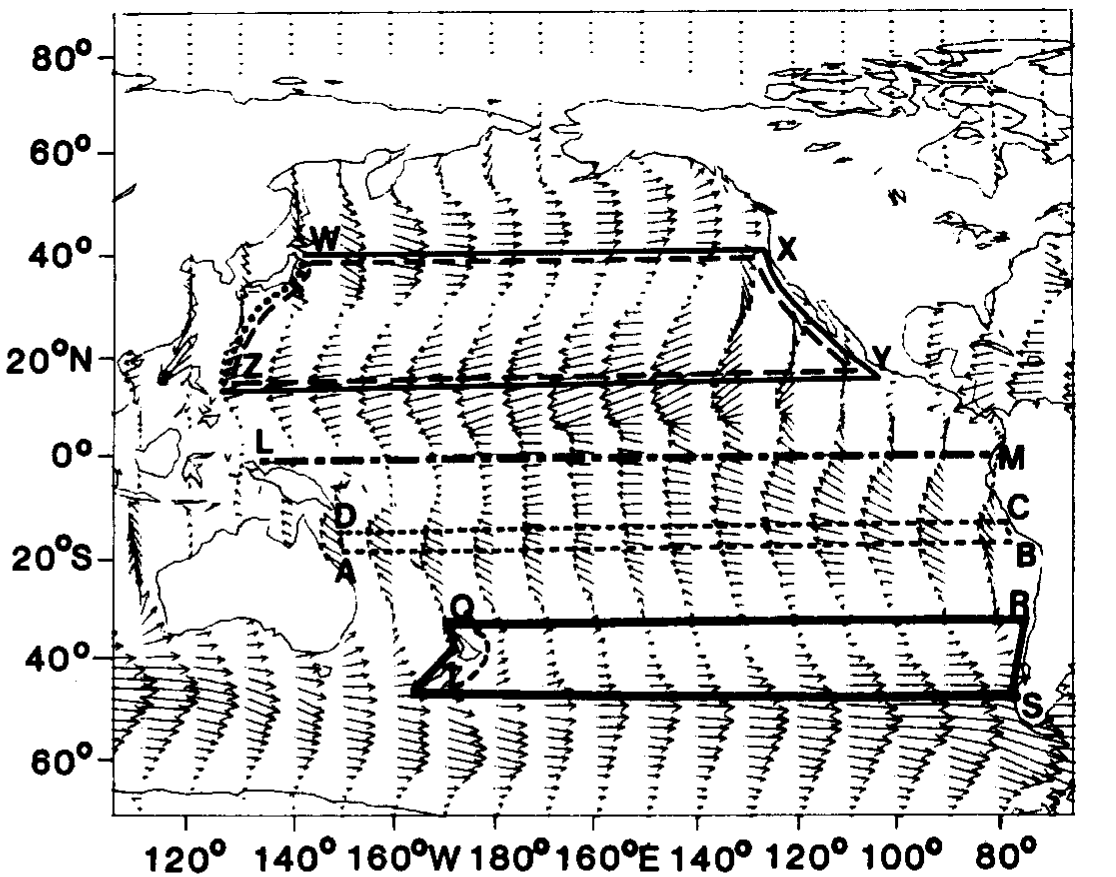
\includegraphics[width=.7\textwidth]{figures/outro/godfrey}
	\end{sidecaption}
\end{figure}

Treating Australasia\sidenote{Consisting of Australia, New Zealand, New Guinea, and some neighboring, minor islands.} as a single island, the Island Rule can even be used to compute an estimate of the \ac{ITF}. --- doing so yields a very realistic magnitude of \SI{16(4)}{\sv} (after \cite{godfrey}).

However, the Island Rule implies that the \ac{ITF} is fed entirely by \emph{southern} water, which contradicts observations (\cf \secref{sec:obs-itf}). Godfrey addresses this in \cite{godfreyind}, proposing the solution that water from the southern hemisphere retroflects into the \ac{NECC} (as seen in the \ac{CESM} experiments), then joins the \ac{NEC} after some time, and ultimately feeds the \ac{ITF} via the \ac{MC}. However, it is still unclear whether this interpretation of the real events holds up.

One further contradiction with the Island Rule is given in \cite{jochumind}, where it is shown that the total transport in the \ac{ITF} decreases when the tip of New Guinea is removed, even though the Island Rule predicts an \emph{increased} transport due to a changed wind stress at the northern edge of its integration part\sidenote[-2]{In a way, reducing boundary layer viscosity in \ac{CESM} may have a similar effect as removing land from the northern coast of New Guinea --- due to a reduced boundary layer width, it also causes the flow to stay further south.}.

All of the previously discussed weak points of the Island Rule come from the same apparent contradiction: \textsl{How can the \ac{ITF} only depend on the atmospheric forcing without taking any kinematic effects into account?} If the Island Rule were strictly valid for the \ac{ITF}, there would be no dependence of the throughflow magnitude on viscosity whatsoever\sidenote[-1]{As long as viscosity does not move the flow path to regions of different wind stress, \ie as long as \(f(Q)\) and \(f(T)\) are taken constant in \eqref{eq:island-rule}.} --- however, in models, at least a slight dependence \emph{is} observed (see \secref{sec:obs-itf} and \eg \cite{jochumind}).

Godfrey already stated in his introductory paper on the Island Rule \citep{godfrey}:

\q{\slshape However, the result does depend critically on the assumption that all
	vorticity entering the western boundary is immediately dissipated, at the latitude
	where it is created.}

For no-slip boundary conditions in a western boundary layer with an interior ocean in Sverdrup balance, Pedlosky states in \citebook{pedloskyoct}:

\q{\slshape [...] in the steady state the vorticity put into the latitude strip (Y1, Y2) by the wind must be locally dissipated in the same latitude band by a horizontal flux of vorticity out of the basin in that same strip.}

However, near the equator, there is no \q{Sverdrup interior} that matches the boundary solution, and nonlinearities become important, so this assumption does not necessarily hold for the \ac{ITF}. It is thus indeed questionable whether the Island Rule may be trusted close to the equator.

\parabreak

\citet{wajsowicz} proposes an extension of the Island Rule for the \ac{ITF} that takes friction and topography into account, and finds an \ac{ITF} transport that is \emph{reduced} by about \SI{2}{\sv}. \citeauthor{wajsowicz}'s model predicts a transport that is generally lower for larger boundary layer widths \(\delta_M\) (and thus higher viscosities), in contrast to what is found in \ac{CESM} (higher \ac{ITF} transport for higher viscosity). The theoretical response described by \citeauthor{wajsowicz} is thus not the effect that is responsible for the behavior in \ac{CESM}.